% 图 57.1 —— 由 `checks/emit_hand.py` 自动拼出（probe 精测 + prims2 图元分解）
%%
% ⚠ 这是**稿子不是成品**：跑 `checks/checkhand.py 57.1` 看指标 + 看叠合图。
%%
%% ⚠ 待核：
%   · 本图 probe 报出阴影族 1 个 —— **本脚本不生成阴影**（要照原书手写）；prims2 的 strokes 里可能含阴影线，核对时留意别画重
%   · 可疑字形 1 项（空心圈 ⊙ 常被认成字母 o）—— 见文件末
%%
\documentclass[12pt]{standalone}
\usepackage{fontspec}
\setsansfont{Arial}
\newfontfamily\mfallback{DejaVu Sans}
\usepackage{tikz}
\begin{document}
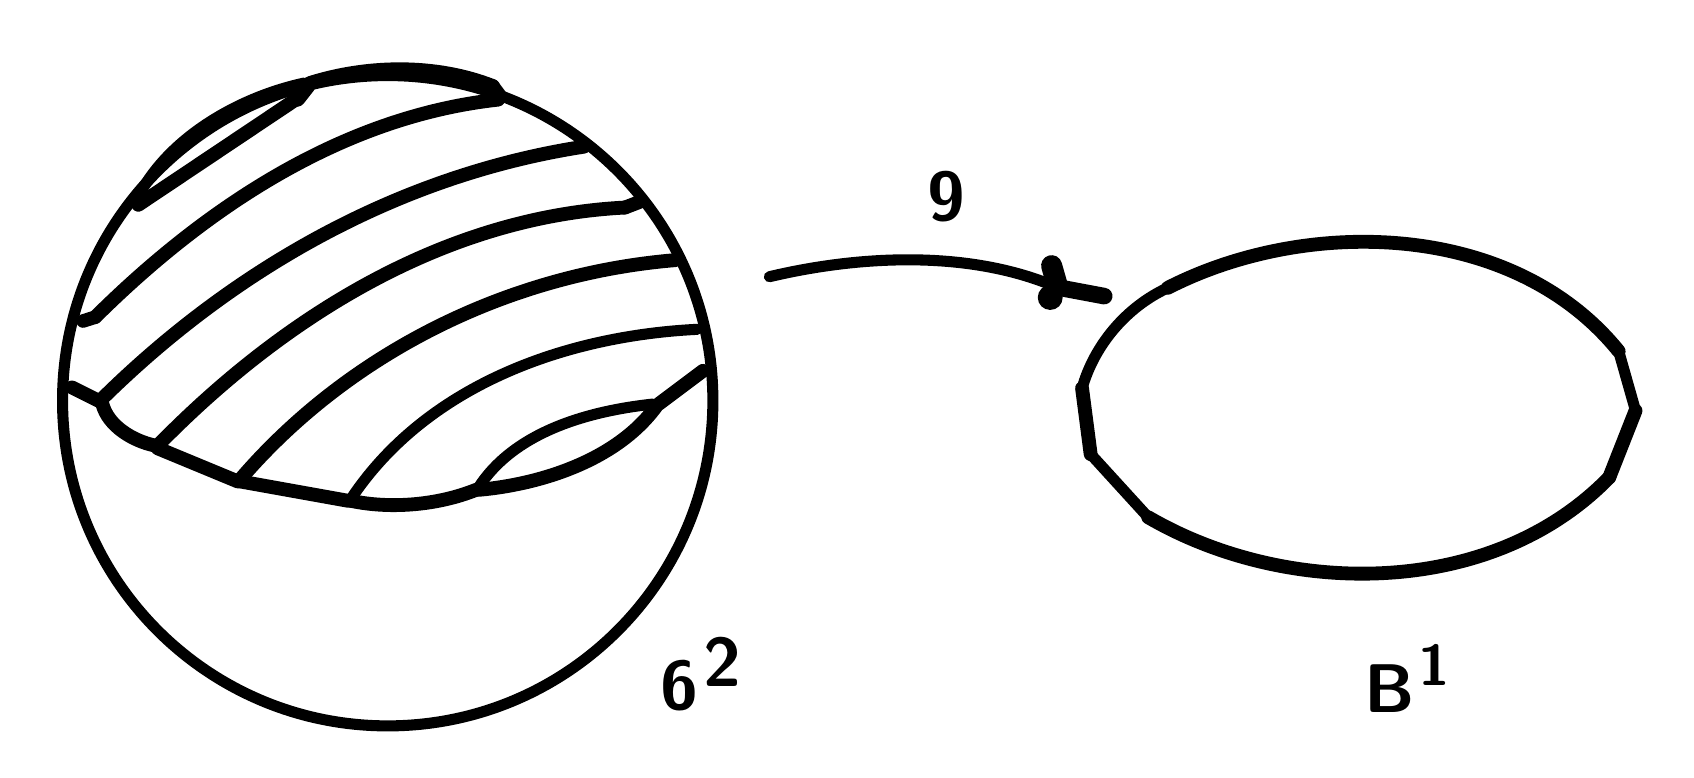
\begin{tikzpicture}[x=1pt, y=-1pt, line width=4.0pt, line cap=round, line join=round]

  %% ════ 填充区（prims2 的 fills）════

  %% ════ 直线段（prims2 的 strokes）════
  \draw[line width=4.9pt] (20.0,106.0) -- (24.4,104.6);
  \draw[line width=5.0pt] (116.0,171.0) -- (77.0,164.0);
  \draw[line width=6.0pt] (389.0,97.0) -- (373.0,94.0);
  \draw[line width=5.0pt] (228.0,136.0) -- (244.0,124.0);
  \draw[line width=4.9pt] (168.1,21.1) -- (171.0,25.0);
  \draw[line width=5.9pt] (101.0,21.0) -- (97.4,25.6);
  \draw[line width=5.0pt] (97.4,25.6) -- (40.0,64.0);
  \draw[line width=5.0pt] (76.0,164.0) -- (47.0,152.0);
  \draw[line width=7.6pt] (370.0,86.0) -- (372.0,93.0);
  \draw[line width=5.0pt] (16.0,130.0) -- (26.0,135.0);
  \draw[line width=5.0pt] (215.8,65.0) -- (221.0,63.0);
  \draw[line width=4.0pt] (574.9,116.9) -- (581.0,138.4);
  \draw[line width=5.0pt] (581.0,138.4) -- (571.5,162.5);
  \draw[line width=4.0pt] (404.9,176.9) -- (384.1,154.1);
  \draw[line width=5.0pt] (384.1,154.1) -- (381.0,130.3);

  %% ════ 曲线（prims2 的 curves —— 三段式，坐标同为 (y,x)）════
  \draw[line width=4.0pt] (242.0,109.0) .. controls (194.9,111.3) and (144.6,128.8) .. (117.0,170.0);
  \draw[line width=5.0pt] (24.4,104.6) .. controls (64.6,64.7) and (114.1,32.1) .. (170.0,26.0);
  \draw[line width=5.0pt] (46.0,151.0) .. controls (38.3,149.4) and (29.1,144.1) .. (27.0,136.0);
  \draw[line width=4.0pt] (268.0,90.0) .. controls (300.4,82.3) and (339.1,80.4) .. (370.0,93.0);
  \draw[line width=5.0pt] (27.0,134.0) .. controls (75.5,86.2) and (135.4,53.1) .. (201.0,43.0);
  \draw[line width=5.0pt] (227.0,137.0) .. controls (212.6,156.5) and (185.2,165.0) .. (163.0,167.0);
  \draw[line width=5.0pt] (102.0,20.0) .. controls (122.9,13.4) and (147.6,13.0) .. (168.1,21.1);
  \draw[line width=4.0pt] (39.0,63.0) .. controls (49.7,40.1) and (76.3,25.1) .. (100.0,20.0);
  \draw[line width=5.0pt] (77.0,163.0) .. controls (116.8,116.8) and (174.6,88.9) .. (234.0,84.0);
  \draw[line width=5.0pt] (47.0,151.0) .. controls (92.0,104.9) and (150.4,68.3) .. (215.8,65.0);
  \draw[line width=5.0pt] (117.0,171.0) .. controls (131.3,174.0) and (148.4,172.5) .. (162.0,167.0);
  \draw[line width=4.0pt] (226.0,136.0) .. controls (202.9,138.5) and (176.2,145.8) .. (163.0,166.0);
  \draw[line width=5.0pt] (412.0,94.0) .. controls (462.2,68.3) and (536.8,69.8) .. (574.9,116.9);
  \draw[line width=5.0pt] (571.5,162.5) .. controls (528.9,206.4) and (454.7,205.9) .. (404.9,176.9);
  \draw[line width=4.0pt] (381.0,130.3) .. controls (385.4,114.7) and (397.0,100.9) .. (412.0,94.0);

  %% ════ 圆 / 椭圆（probe 精测）════
  \draw (130.1,134.8) circle (117.5);

  %% ════ 实心点 ════
  \fill (369.5,97.5) circle (4.5);

  %% ════ 标签（probe 直接给的 \node 行）════
  %% ⚠ 全部补了 fill=white：文字在最上层，否则与曲线交叉干扰
     \node[anchor=center,inner sep=0pt,fill=white,font=\fontsize{34.0}{42.5}\selectfont] at (332.0,60.9) {\textsf{\textbf{9}}};   % box(321,49,18,22)
     \node[anchor=center,inner sep=0pt,fill=white,font=\fontsize{22.9}{28.7}\selectfont] at (251.1,229.4) {\textsf{\textbf{2}}};   % box(245,221,11,16)
     \node[anchor=center,inner sep=0pt,fill=white,font=\fontsize{22.2}{27.8}\selectfont] at (508.1,230.4) {\textsf{\textbf{1}}};   % box(502,222,7,16)
     \node[anchor=center,inner sep=0pt,fill=white,font=\fontsize{36.5}{45.6}\selectfont] at (235.4,237.9) {\textsf{\textbf{6}}};   % box(225,225,19,24)
     \node[anchor=center,inner sep=0pt,fill=white,font=\fontsize{30.2}{37.8}\selectfont] at (492.3,239.0) {\textsf{\textbf{\textit{B}}}};   % box(481,227,19,23)

  % 钉死画布：否则超出的图元/控制点会把页面撑大，1:1 回比就失准
  \pgfresetboundingbox
  \path[use as bounding box] (0,0) rectangle (592,261);
\end{tikzpicture}
\end{document}

% ⚠ 待核清单（probe 拿不准，人眼过一遍）：
%   · 未识别/跳过：⑤ 跳过/未识别的字形
